\begin{frame}
	\begin{columns}
		\column{0.6\textwidth}
		\begin{overlayarea}{\textwidth}{\textheight}
			\onslide<1->{
				\begin{itemize}\justifying
					\item<1-> Let us fix the threshold ($-w_0 = 1$) and try different values of $w_1, w_2$
					\item<2-> Say, $w_1=-1, w_2=-1$
					\item<3-> What is wrong with this line? \onslide<4->{We make an error on 1 out of the 4 inputs}
					\item<5-> Lets try some more values of $w_1, w_2$ and note how many errors we make

					      \onslide<6->{
						      \begin{center}
							      \begin{table}
								      \begin{tabular}{ccc}
									      \hline
									      $w_1$              & $w_2$              & errors          \\
									      \hline
									      \onslide<6->{-1}   & \onslide<6->{-1}   & \onslide<6->{1} \\
									      \onslide<7->{1.5}  & \onslide<7->{0}    & \onslide<7->{1} \\
									      \onslide<8->{0.45} & \onslide<8->{0.45} & \onslide<8->{3} \\
									      \hline

									      \hline
								      \end{tabular}
							      \end{table}
						      \end{center}
					      }
					\item<9-> We are interested in those values of $w_0, w_1, w_2$ which result in 0 error
					\item<10-> Let us plot the error surface corresponding to different values of $w_0, w_1, w_2$
				\end{itemize}
			}
		\end{overlayarea}

		\column{0.4\textwidth}
		\begin{overlayarea}{\textwidth}{\textheight}
			\begin{center}
				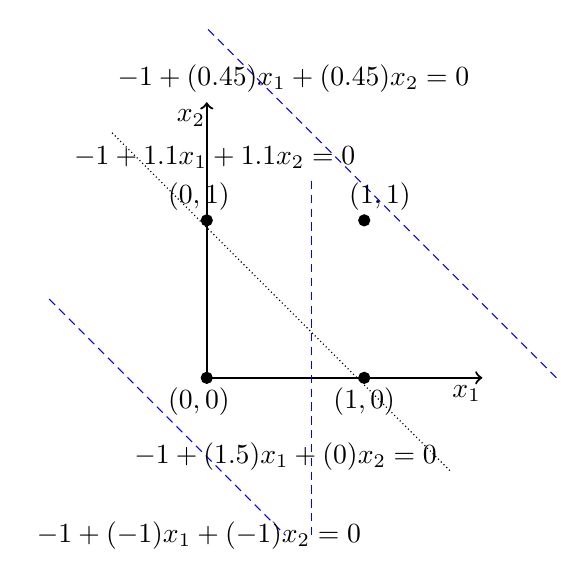
\begin{tikzpicture}

	\draw[thick,->] (0,0) -- (3.5,0);
	\draw[thick,->] (0,0) -- (0,3.5);

	\onslide<1->{\draw[densely dotted] (-1.2021,3.1111) -- (3.1111,-1.2021);}
	\onslide<2->{\draw[densely dashed, blue] (-2,1) -- (1,-2);}
	\onslide<7->{\draw[densely dashed, blue] (1.33,2.5) -- (1.33,-2.0);}
	\onslide<8->{\draw[densely dashed, blue] (4.44,0) -- (0,4.44);}

	\node at (3.3, -0.2) {$x_1$};
	\node at (-0.2, 3.3) {$x_2$};

	\node at (-0.1, -0.3) {$(0,0)$};
	\node at (-0.1, 2.3) {$(0,1)$};
	\node at (2.0, -0.3) {$(1,0)$};
	\node at (2.2, 2.3) {$(1,1)$};
	\onslide<1->{\node at (0.1, 2.8) {$-1 + 1.1x_1 + 1.1x_2 = 0$};}
	\onslide<2->{\node at (-0.1, -2.0) {$-1 + (-1)x_1 + (-1)x_2 = 0$};}
	\onslide<7->{\node at (1, -1.0) {$-1 + (1.5)x_1 + (0)x_2 = 0$};}
	\onslide<8->{\node at (1.1, 3.8) {$-1 + (0.45)x_1 + (0.45)x_2 = 0$};}

	\filldraw (0,0) circle (2pt);
	\filldraw (0,2) circle (2pt);
	\filldraw (2,0) circle (2pt);
	\filldraw (2,2) circle (2pt);
\end{tikzpicture}
			\end{center}
		\end{overlayarea}
	\end{columns}
\end{frame}

\begin{frame}
	\begin{columns}
		\column{0.5\textwidth}
		\begin{overlayarea}{\textwidth}{\textheight}
			\begin{figure}
				\includegraphics<4->[scale= 0.5]{images/module4/or_error_surface.png}
			\end{figure}
		\end{overlayarea}

		\column{0.5\textwidth}
		\begin{overlayarea}{\textwidth}{\textheight}
			\begin{itemize}\justifying
				\item<1-> For ease of analysis, we will keep $w_0$ fixed (-1) and plot the error for different values of $w_1, w_2$
				\item<2-> For a given  $w_0, w_1, w_2$ we will compute $-w_0 + w_1*x_1 + w_2*x_2$ for all computations of $(x_1, x_2)$ and note down how many errors we make
				\item<3-> For the OR function, an error occurs if $(x_1, x_2) = (0,0)$  but $-w_0 + w_1*x_1 + w_2*x_2 \geq 0$ or if $(x_1, x_2) \neq (0,0)$  but $-w_0 + w_1*x_1 + w_2*x_2 < 0$
				\item<5-> We are interested in finding an algorithm which finds the values of $w_1, w_2$ which minimize this error
			\end{itemize}
		\end{overlayarea}
	\end{columns}
\end{frame}

